\section{Séance 2}
\paragraph{1. } Dans le graphe ci-dessous, trouvez le nombre de parcours fermés contenant le point $A$.

\begin{figure}[h!]
  \begin{center}
    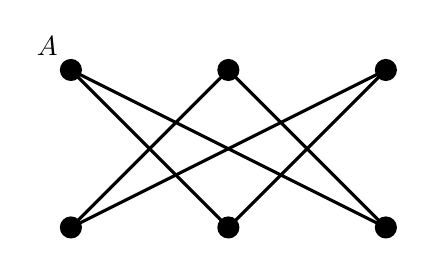
\begin{tikzpicture}[scale=1,looseness=1,auto,line width=.4mm]

      \path[draw=none] (-2.3,1.3) node { $A$ };

      \draw (-2, 1) -- ( 0,-1);
      \draw (-2, 1) -- ( 2,-1);
      \draw ( 0, 1) -- (-2,-1);
      \draw ( 0, 1) -- ( 2,-1);
      \draw ( 2, 1) -- (-2,-1);
      \draw ( 2, 1) -- ( 0,-1);

      \draw[fill=black] (-2,-1) circle(.12);
      \draw[fill=black] (-2, 1) circle(.12);
      \draw[fill=black] ( 0,-1) circle(.12);
      \draw[fill=black] ( 0, 1) circle(.12);
      \draw[fill=black] ( 2,-1) circle(.12);
      \draw[fill=black] ( 2, 1) circle(.12);

    \end{tikzpicture}
  \end{center}
\end{figure}
\vspace{-1cm}

\paragraph{2. } Est-il possible de tracer les figures suivantes sans lever le crayon et sans passer deux fois par le même segment?

\begin{figure}[h!]
  \begin{center}
    \begin{tabular}{lcccr}
      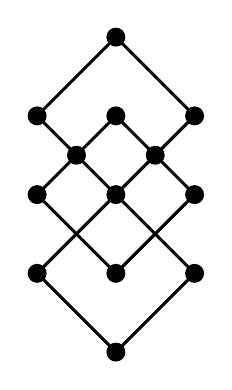
\begin{tikzpicture}[scale=1,looseness=1,auto,line width=.4mm]

        \draw (-1, 1) -- (  0, 2);
        \draw (-1, 1) -- (-.5,.5);
        \draw (-1, 0) -- (  0,-1);
        \draw (-1, 0) -- (-.5,.5);
        \draw (-1,-1) -- (  0, 0);
        \draw (-1,-1) -- (  0,-2);
        \draw ( 1, 1) -- (  0, 2);
        \draw ( 1, 1) -- ( .5,.5);
        \draw ( 1, 0) -- (  0,-1);
        \draw ( 1, 0) -- ( .5,.5);
        \draw ( 1,-1) -- (  0, 0);
        \draw ( 1,-1) -- (  0,-2);
        \draw ( 0, 0) -- ( .5,.5);
        \draw ( 0, 0) -- (-.5,.5);
        \draw ( 0, 1) -- ( .5,.5);
        \draw ( 0, 1) -- (-.5,.5);

        \draw[fill=black] ( -1, 1) circle(.1);
        \draw[fill=black] ( -1, 0) circle(.1);
        \draw[fill=black] ( -1,-1) circle(.1);
        \draw[fill=black] (  0,-2) circle(.1);
        \draw[fill=black] (  0,-1) circle(.1);
        \draw[fill=black] (  0, 0) circle(.1);
        \draw[fill=black] (  0, 1) circle(.1);
        \draw[fill=black] (  0, 2) circle(.1);
        \draw[fill=black] (  1, 1) circle(.1);
        \draw[fill=black] (  1, 0) circle(.1);
        \draw[fill=black] (  1,-1) circle(.1);
        \draw[fill=black] (-.5,.5) circle(.1);
        \draw[fill=black] ( .5,.5) circle(.1);

      \end{tikzpicture}
      & \hspace{1cm} &
      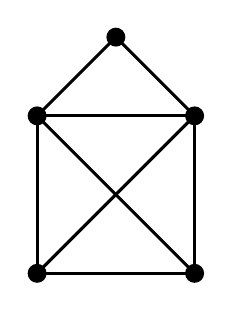
\begin{tikzpicture}[scale=1,looseness=1,auto,line width=.4mm]

        \draw (0,0) -- (2,0);
        \draw (0,0) -- (2,2);
        \draw (0,0) -- (0,2);
        \draw (2,0) -- (2,2);
        \draw (2,0) -- (0,2);
        \draw (0,2) -- (2,2);
        \draw (0,2) -- (1,3);
        \draw (2,2) -- (1,3);

        \draw[fill=black] (0,0) circle(.1);
        \draw[fill=black] (2,0) circle(.1);
        \draw[fill=black] (2,2) circle(.1);
        \draw[fill=black] (0,2) circle(.1);
        \draw[fill=black] (1,3) circle(.1);

      \end{tikzpicture}
      & \hspace{1cm} &
      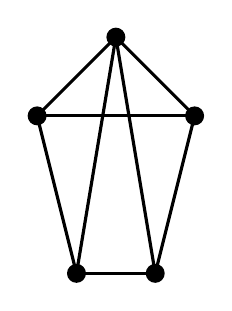
\begin{tikzpicture}[scale=1,looseness=1,auto,line width=.4mm]

        \draw (.5,0) -- (1.5,0);
        \draw (.5,0) -- (1,3);
        \draw (.5,0) -- (0,2);
        \draw (1.5,0) -- (2,2);
        \draw (1.5,0) -- (1,3);
        \draw (0,2) -- (2,2);
        \draw (0,2) -- (1,3);
        \draw (2,2) -- (1,3);

        \draw[fill=black] (.5,0) circle(.1);
        \draw[fill=black] (1.5,0) circle(.1);
        \draw[fill=black] (2,2) circle(.1);
        \draw[fill=black] (0,2) circle(.1);
        \draw[fill=black] (1,3) circle(.1);

      \end{tikzpicture}
    \end{tabular}
  \end{center}
\end{figure}
\vspace{-1cm}

\paragraph{3. } En vous basant sur la preuve inductive du théorème qui caractérise les graphes eulériens, décrivez un algorithme qui trouve un circuit eulérien en un temps $O(|E|)$.

\paragraph{4. } \textbf{Séquences de de Bruijn.} Le problème suivant apparaît sous de nombreuses formes. On demande de construire la plus longue séquence circulaire de lettres d'un alphabet de $k$ lettres sans qu'aucune sous-séquence de longueur $n$ ne soit répétée.
\begin{enumerate}
  \item Donnez une borne supérieure sur la longueur de la séquence circulaire en question.
  \item Cette borne peut-elle être atteinte? Formulez cette question comme un problème de tour eulérien dans un graphe orienté. (Indice~: les sommets correspondent aux séquences de longueur $n-1$ et les arêtes aux séquences de longueur $n$.)
  \item Pour l'alphabet $\mathcal{A} = \{0, 1, 2\}$ de $k = 3$ lettres et pour $n = 3$, répondez à la question précédente en construisant la plus longue séquence circulaire.
\end{enumerate}

\newpage

\paragraph{5. } On souhaite trouver un parcours fermé de poids minimum passant au moins une fois par chaque arête du graphe suivant~:
\begin{figure}[h!]
  \begin{center}
    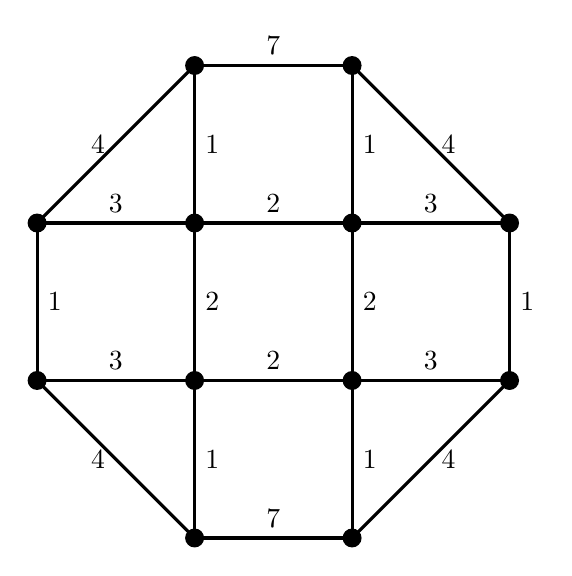
\begin{tikzpicture}[scale=1,auto,line width=.4mm]

      \coordinate (11++) at ( 1, 1);
      \coordinate (13++) at ( 1, 3);
      \coordinate (31++) at ( 3, 1);
      \coordinate (11+-) at ( 1,-1);
      \coordinate (13+-) at ( 1,-3);
      \coordinate (31+-) at ( 3,-1);
      \coordinate (11-+) at (-1, 1);
      \coordinate (13-+) at (-1, 3);
      \coordinate (31-+) at (-3, 1);
      \coordinate (11--) at (-1,-1);
      \coordinate (13--) at (-1,-3);
      \coordinate (31--) at (-3,-1);

      \draw (11++) -- (13++) node[midway,right] {$1$};
      \draw (11++) -- (31++) node[midway,above] {$3$};
      \draw (31++) -- (13++) node[midway,above,right] {$4$};
      \draw (11+-) -- (13+-) node[midway,right] {$1$};
      \draw (11+-) -- (31+-) node[midway,above] {$3$};
      \draw (31+-) -- (13+-) node[midway,below,right] {$4$};
      \draw (11-+) -- (13-+) node[midway,right] {$1$};
      \draw (11-+) -- (31-+) node[midway,above] {$3$};
      \draw (31-+) -- (13-+) node[midway,above,left] {$4$};
      \draw (11--) -- (13--) node[midway,right] {$1$};
      \draw (11--) -- (31--) node[midway,above] {$3$};
      \draw (31--) -- (13--) node[midway,below,left] {$4$};
      \draw (11++) -- (11+-) node[midway,right] {$2$};
      \draw (11++) -- (11-+) node[midway,above] {$2$};
      \draw (11--) -- (11+-) node[midway,above] {$2$};
      \draw (11--) -- (11-+) node[midway,right] {$2$};
      \draw (13++) -- (13-+) node[midway,above] {$7$};
      \draw (13+-) -- (13--) node[midway,above] {$7$};
      \draw (31++) -- (31+-) node[midway,right] {$1$};
      \draw (31-+) -- (31--) node[midway,right] {$1$};

      \draw[fill=black] (11++) circle(.1);
      \draw[fill=black] (13++) circle(.1);
      \draw[fill=black] (31++) circle(.1);
      \draw[fill=black] (11+-) circle(.1);
      \draw[fill=black] (13+-) circle(.1);
      \draw[fill=black] (31+-) circle(.1);
      \draw[fill=black] (11-+) circle(.1);
      \draw[fill=black] (13-+) circle(.1);
      \draw[fill=black] (31-+) circle(.1);
      \draw[fill=black] (11--) circle(.1);
      \draw[fill=black] (13--) circle(.1);
      \draw[fill=black] (31--) circle(.1);

    \end{tikzpicture}
  \end{center}
\end{figure}
\vspace{-1cm}

\paragraph{6. } Dans le graphe suivant, trouvez un chemin de coût minimum du sommet $1$ au sommet $7$. Le chemin doit traverser toutes les arêtes au moins une fois.
\begin{figure}[h!]
  \begin{center}
    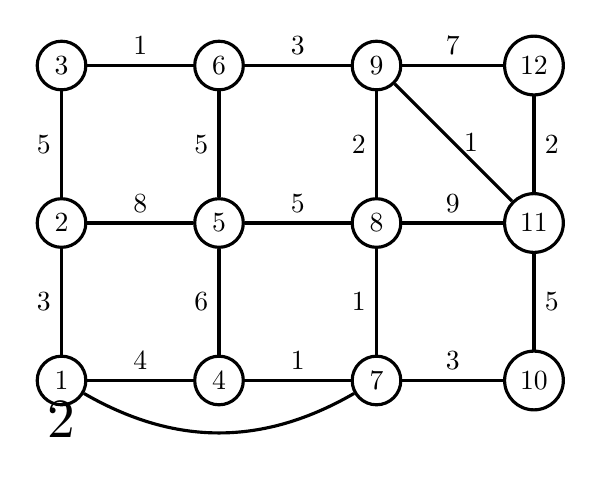
\begin{tikzpicture}[scale=2,auto,line width=.4mm]

      \path (0,0) node[draw,shape=circle] (1)  {$1$};
      \path (0,1) node[draw,shape=circle] (2)  {$2$};
      \path (0,2) node[draw,shape=circle] (3)  {$3$};
      \path (1,0) node[draw,shape=circle] (6)  {$4$};
      \path (1,1) node[draw,shape=circle] (5)  {$5$};
      \path (1,2) node[draw,shape=circle] (4)  {$6$};
      \path (2,0) node[draw,shape=circle] (7)  {$7$};
      \path (2,1) node[draw,shape=circle] (8)  {$8$};
      \path (2,2) node[draw,shape=circle] (9)  {$9$};
      \path (3,0) node[draw,shape=circle] (12) {$10$};
      \path (3,1) node[draw,shape=circle] (11) {$11$};
      \path (3,2) node[draw,shape=circle] (10) {$12$};

      \draw (1)  -- (2)  node[midway,left]  {$3$};
      \draw (2)  -- (3)  node[midway,left]  {$5$};
      \draw (6)  -- (5)  node[midway,left]  {$6$};
      \draw (5)  -- (4)  node[midway,left]  {$5$};
      \draw (7)  -- (8)  node[midway,left]  {$1$};
      \draw (8)  -- (9)  node[midway,left]  {$2$};
      \draw (12) -- (11) node[midway,right] {$5$};
      \draw (11) -- (10) node[midway,right] {$2$};
      \draw (1)  -- (6)  node[midway,above] {$4$};
      \draw (2)  -- (5)  node[midway,above] {$8$};
      \draw (3)  -- (4)  node[midway,above] {$1$};
      \draw (4)  -- (9)  node[midway,above] {$3$};
      \draw (5)  -- (8)  node[midway,above] {$5$};
      \draw (6)  -- (7)  node[midway,above] {$1$};
      \draw (7)  -- (12) node[midway,above] {$3$};
      \draw (8)  -- (11) node[midway,above] {$9$};
      \draw (9)  -- (10) node[midway,above] {$7$};
      \draw (9)  -- (11) node[midway,above,right] {$1$};
      \draw (1) to[bend right] (7) node[midway,below] {$2$};

    \end{tikzpicture}
  \end{center}
\end{figure}
\vspace{-1cm}

\paragraph{7. } Résolvez le problème du postier chinois sur l'hypercube de dimension $k$.
